\documentclass[../main.tex]{subfiles}
\graphicspath{{\subfix{../IMAGES/}}}

\begin{document}
\localtableofcontents
\subsection{Introduction}
Proton : Particule dans noyau, charge $p^+$ masse : $1.6727\cdot 10^{-24}$g\\
Électrons : Particule autour du noyau, charge $e^-$ masse : $9.11\cdot 10^{-28}$g\\
Neutron : Particule dans le noyau, pas de charge, masse : $1.675\cdot 10^{-27}$g.\\

Électrons sont importants dans les liaisons chimiques. Source de la conductivité électrique. Interaction forte au champ électrique et magnétique. \\
La lumière est une onde électromagnétique qui résulte du mouvement des charges électriques. Dans le vide : $\lambda f = c = \frac{1}{\sqrt{\varepsilon_0 \mu_0}} = 3\cdot 10^8m\cdot s^{-1}$.\\
Énergie du photon [J] : $E = hf$. On a émission de lumière si atome passe de niveau excité à niveau fondamental. \\
L'état d'énergie est définit par : $E_n = \frac{-13.6 eV}{n^2}$. Avec la constante de Rydberg $R_{\infty}$ : $\frac{1}{\lambda} = R_{\lambda} (\frac{1}{n_1^2}- \frac{1}{n_2^2})$.\\
De plus, on a $\lambda = \frac{h}{mf}$, avec h: constante de plack : $6.63\cdot 10^{-34}J\cdot s$\\
Selon Schrödinger : orbitales des atomes sont définies par 3 nombre entier n,l,$m_l$:\\
\textbf{n : nombre quantique principale} n$\geq$1 (taille et énergie de l'orbitale)\\
\textbf{l : nombre quantique angulaire} $0\leq l \leq n-1$ (forme de l'orbitale)\\
\textbf{$m_l$ : nombre quantique magnétique} $-l \leq m_l \leq l$ (orientation de l'orbitale)\\
\textbf{$m_s$ : nombre quantique de spin} $\frac{1}{2}$ ou $-\frac{1}{2}$\\

\quad \underline{Règle de Klechkowski :}\\
\begin{minipage}{.3\textwidth}
    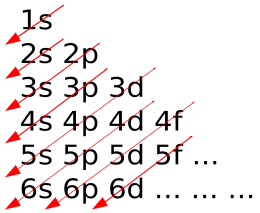
\includegraphics[width=\textwidth]{IMAGES/mx/260px-Klechkovski_rule.svg.png}
\end{minipage}
\hfill
\begin{minipage}{.7\textwidth}
    \underline{Principe de Pauli :} 1 orbitale possède 2 électrons maximum et sont de spins opposés.\\
    Dans un atome, chaque électron est défini par un groupe différents (n,l,$m_l$,$m_s$)\\

    \underline{Règle de Hund :} L'arrangement le plus stable est celui où il y a un maximum d'électrons de spins parallèles.
\end{minipage}

Électrons de valence : ce sont ceux qui occupent la couche ayant la plus grande valeur de n. (déterminent les propriétés chimiques des éléments).\\

\quad \underline{Tableau périodique des éléments (Mendeleiev :}\\
Construit selon principe de Aufbau : on ajoute un électron et un proton pour passer à l'élément suivant. Le numéro atomique Z donne le nombre de proton (nombre d'électrons). Le nombre de masse A donne le nombre de nucléons (proton plus neutrons).\\

\underline{Isotope : } des atomes avec le même nombre de protons mais nombre d'électrons différents.\\

Sur le tableau, 92 éléments naturels, les autres sont artificiels. Les éléments dans une même colonne appartiennent à un même groupe (ex : métaux) et ont le même nombre d'électrons de valence. Les lignes sont les périodes.\\
Le rayon atomique \textbf{augmente} en passant d'une période à une autre et \textbf{diminue} quand la charge du noyau augmente.\\

\quad \underline{Énergie d'ionisation :}
Énergie pour extraire un électron. \\

\quad \underline{Electroaffinité :}
Variation d'énergie lors de la capture d'un électron. \\

\quad \underline{Interaction entre atomes :}
Atomes interagissent entre eux pour former des interactions durables en fonction de température et pression. On modélise leur interaction comme des ressorts. \\
Potentiel de Lennard Jones : $E = \varepsilon_0 [(\frac{r_0}{r})^{12}-2(\frac{r_0}{r})^6]$\\
Pendant les réactions, les éléments chimiques se combinent et en forment d'autre plus stable énergétiquement. \\
\textbf{On a toujours conservation de la masse!} Différents types de réactions : $\rightleftharpoons$ (en équilibre/réaction dans les deux sens); $\Rightarrow$ (complète).\\
\underline{Mole : } quantité de substance contenant le même nombre d'atomes que 12g de carbone 12 pur.\\

\subsection{Liaisons chimiques}


\quad \underline{Polarité des liaisons :}\\
force attractive d'un atome dans une liaison est quantifié par son électronégativité. Dipôle va du moins électronégatif vers le plus.\\

\quad \underline{Liaisons ioniques :}
Dans les métaux/non-métaux. Des cations et anions se forment. Les électrons de valences vont des métaux vers les non-métaux. Liaisons non directionnelles. \textbf{Liaisons entre deux ions si $\Delta EN > 1.67$}. Les cations sont plus petits que les anions en général.\\ 
Arrangement d'anions et cations en réseau réguliers pour obtenir un système d'énergie minimum. Liaisons fortes et point de fusion élevé. \\

\quad \underline{Liaisons covalentes :}\\
Liaisons directionnelles. Dans non-métaux/non-métaux. Atomes partagent un ou plusieurs électrons de valence. Entre deux atomes de même nature. Les atomes combinent leur orbitales en un état liant et un anti-liant. \\
Existe si $\Delta EN < 1.67$. \\

\quad \underline{Liaisons métalliques :}
La plupart des éléments à l'état natif sont des métaux. Ils partagent leur électrons de valence. \\

\quad \underline{Liaisons intermoléculaires (faibles) :}\\
Forces intermoléculaires plus faible que les liaisons intramoléculaire. Elles déterminent les propriétés physiques macroscopiques des liquides et des solides. De plusieurs sortes :\\
Forces ion-dipôle : détermine la solubilité, fortes pour petits ions très chargés.\\
Forces dipôle-dipôle : entre molécules polaire, font orienter les atomes.\\
Forces de london : attraction entre dipôle instantanés sur des molécules voisines.\\
Liaisons hydrogène : un atome hydrogène entre deux atomes très électronégatif.\\

\quad \underline{Cas du carbone :}\\
\qquad \underline{Hybridation du carbone :}\\
$sp^3$ : (liaison simple) molécule en 3D : exemple méthane\\
$sp^2$ : (liaison double) molécule en 2D : exemple éthylène\\
$sp$ : (liaison triple) molécule linéaire\\


\quad \underline{Liaisons délocalisée : benzène }\\
Pour du benzène, orbitales 2p sont en dehors du plan et peuvent donc interagir librement. Chaque électrons n'est pas attaché à un atome ou une liaison mais est délocalisé. Renforce les liaisons. \\

\subsection{États des corps solides}
\quad \underline{État vitreux :}\\
Celui d'un liquide figé avec une grande viscosité. N'a pas le temps de s'organiser pendant le refroidissement pour réduire le volume; n'a pas pu cristalliser. Même un métal peut être sous forme amorphe.\\

\quad \underline{État cristallin :}
Il est ordonné et décrit un motif qui se répète à chaque noeud d'un réseau cristallin.\\
On peut représenter un réseau cristallin en 3D avec trois vecteurs a,b et c pour avoir une maille dans l'espace. Sur chaque noeud, le cristal apparaît identique. Il y a une invariance par translation le long des vecteurs a,b et c.\\
Il existe 7 réseaux cristallins et 14 réseaux de Bravais. Un cristal est un motif + un réseau de Bravais. Les trois réseaux les plus connus : Cubique Simple (CS), Cubique centré (CC), Cubique Face Centrée (CFC). Pour désigner une direction réticulaire (qui forme un réseau) et un plan réticulaire on utilise les \textbf{indices de Miller}. \\

Décrire un plan de réseau : (x,y,z) : inverse des coordonnées des intersection du plan avec les axes définissant la structure. \\
$[x,y,z] $: composantes du vecteur colinéaire à cette direction et qui passe par l'origine.\\

Paramètre de maille : a (longueur d'un côté).\\
$\rho = \frac{m_{at} N_{b atome/maille}}{V_{maille}} kg.m^{-3}$\\
Compacité : $C = \frac{V_{at} N_{b atome/maille}}{V_{maille}}$\\

\quad \underline{Diffraction :}
Ondes sont réfléchies sur une surface et l'angle de réflexion est le même que l'angle incident. Si le $\lambda$ est le même ordre de grandeur que la distance entre plan inter-atomiques, les ondes interfèrent avec ces plans.\\

\underline{Lois de Bragg :} Ondes sont constructives si la différence de chemin optique est un multiple de $\lambda$. $2l = 2d sin\theta = n\lambda$.\\

\subsubsection{Différentes notions}
\quad \underline{Nombre de coordination :}\\
Nombre de voisins proche à chaque atome (liaison directe)\\

\quad \underline{Plans empilement compacte :}\\
Plan selon lequel les atomes sont le plus serrés.\\

Réseau CFC : 26\% de vide, CC : 32\% de vide\\

\quad \underline{Défauts :}
Le cristal parfait n'existe pas. Il y a plusieurs types de défauts : lacune (il manque un atome), défaut ponctuel substitutionnel (1 atome remplacé par un autre), défaut ponctuel interstitiel (1 atome vient au milieu des autres), dislocations.\\
Beaucoup de matériaux sont polycristallins et sont multiphasés. \\

\quad \underline{Sites interstitiels du CFC :}
Atomes de solutés vont se loger dans les sites interstitiels. Pour les mailles de CFC il y a deux sites : au centre de la maille et dans les site tétrahédrique (à $\frac{1}{4}$ des diagonales du cube).\\

\quad \underline{Structure des céramiques :}\\
Liaisons ioniques, les céramiques ont une structure compacte et plus complexe que les métaux. \\

\quad \underline{Structure des matériaux organiques :}\\
Polymère : un motif de base répété. Polymérisation : opération pour passer d'une molécule simple à une macromolécule. Masse molaire : $M_i = i M_{molaire}$ avec i : le degré de polymérisation.\\

Deux catégories : \textbf{homopolymères} un seul bloc de base A. \textbf{Copolymère} deux blocs de base A et B.\\
Trois sortes : linéaire, branché, réticulé. \\
Thermoplastiques : polymères moulé à chaud/amorphe ou semi-cristallin\\
Élastomères : polymères réticulé à chaud pour avoir une grande élasticité : amorphes et non-recyclables. \\

\subsection{Elasticité linéaire}
La raideur : $E = \frac{72 \varepsilon_0}{r_0^3}$\\

On a en traction : $\sigma = \frac{F}{S}$, la contrainte donnée par la force F sur la section S du matériaux. \\

\underline{La déformation :} lorsqu'un corps est soumis à des contraintes, il se déforme. On définit l'élongation par : $\varepsilon = \frac{\Delta L}{L}$ exprimée en \% sans unité.


\quad \underline{Traction/compression uniaxiale :}
Pour des déformations élastique : un corps déformé revient à sa position originale. On définit le \textbf{module d'élasticité/ de Young E}. On a :\\
\begin{equation}
    \sigma = E \varepsilon
\end{equation}
De plus, les efforts dans une dimensions entraînent des efforts et donc des déformations dans les autres. On définit donc \textbf{le module de Poisson $\nu$} : \\
\begin{equation}
    \varepsilon_y = -\nu \varepsilon_x
\end{equation}
 Un changement de volume s'opère donc et on a :\\
 \begin{equation}
     \frac{\Delta V}{V} = \varepsilon_x (1-2\nu)
 \end{equation}
\textbf{$0<\nu<\frac{1}{2}$}\\

Énergie élastique : $W = E \frac{\varepsilon_x^2}{2} V \Rightarrow dW = \sigma_x d\varepsilon_x[J;m^{-3}]$\\

\quad \underline{Compression hydrostatique :} Correspond à une contrainte constante sur toute la surface du solide\\
coefficient k : $k= -V_0 \frac{\Delta p}{\Delta V}[pa]$\\

\quad \underline{Cisaillement simple :}\\
Module de cisaillement G : $\sigma_{xy} = 2G \varepsilon_{xy} = G\gamma = G \frac{\Delta L_x}{L_{0y}}$\\
Solide isotrope : même propriété dans toutes les directions. \\

\quad  \underline{Anisotropie des propriété élastique :}
E, v, G peuvent dépendre de l'orientation : ils sont alors anisotropes. \\

\quad \underline{Plasticité des matériaux :}\\
Déformation élastique : matériaux revient à sa forme initial une fois la contrainte enlevée.\\
Déformation plastique : $\sigma > \sigma_e$ matériaux ne retourne pas à sa forme initial.\\

En déformation plastique, la limite élastique augmente : écrouissage. Ductilité : déformation à la rupture. \\
E est une constante qui dépend de la micro-structure. \\

\subsection{Mécanisme et plasticité des matériaux :}
Dislocations : principal défaut responsable de la plasticité des matériaux. Les défauts d'empilements facilitent la plasticité. \\
2 types de dislocations : vis : cristal coupé en 2 et poussé partiellement d'une rangée. Moins utilisée.\\
Coin : ligne de dislocation délimite la discontinuité. Vecteur de Burgers : correspond à la déformation élémentaire. Celle des coins est la plus impliquée dans déformation plastique des métaux.\\


\quad \underline{Durcissement des métaux :}
Pour augmenter la résistance du matériaux : il faut bloquer le déplacement des dislocations. \\
Plusieurs méthodes : solution solide : mettre des atomes dans la maille; par dislocations; réduire la taille des grains; être polycristallin. \\

\quad \underline{Plasticité des polymères et mécanismes :}\\
Le comportement des polymères dépend de la température et de la vitesse de transformation. En dessous de .75$T_g$ (température transition vitreuse) il est fragile. Au dessus il a un comportement ductile. \\
Pendant la traction, au dessus de .75$T_g$, on a du cisaillement et des craquelures alors qu'en compression uniquement craquelures. \\

\quad \underline{Propriétés des céramiques :}
Céramiques sont fragiles en traction mais très résistant à la compression. \\

\subsection{Dureté des matériaux}
Pour comparer les matériaux on peut faire un test de dureté : Rockwell/Brinell.\\
$\sigma_{vickers} \simeq 10H_v$.\\

\quad \underline{Ténacité :}\\
Résistance à la déformation plastique n'est pas tout beaucoup de problèmes sont dues à la propagation rapide des fissures. \\
On suppose un matériaux avec une fissure traversante de longueur l et d'épaisseur e. On définit le \textbf{facteur d'intensité de contrainte k} correspond à un surplus d'énergie élastique que doit soutenir le restant du matériaux. \\
\begin{equation}
    k = \sigma \sqrt{\pi l}
\end{equation}
Pour faire avancer la fissure il faut casser les liaisons inter-atomiques et créer deux surfaces. Ainsi l'énergie s'opposant à l'avance de la fissure : $W_{\gamma} = 2\gamma le$\\
Ainsi \textbf{la longueur critique de la fissure : $l_c = \frac{2\gamma E}{\pi \sigma^2}$}.\\
Plus un matériaux est fragile : plus sa ténacité est faible. \\
Les métaux CFC restent toujours ductiles mais les autres métaux et tous les polymères voient leur $\sigma$ augmenter si la température diminue. Leur zone ductile diminue et on a une transition rupture ductile/fragile.\\

\subsection{Fatigue}
Même lors de déformation plastique, le matériaux peut se rompre par fatigue. \\
Si $\sigma > \sigma_y$ : low cycle : endommagement rapide\\
Sinon high cycle : peut supporter grand nombre de cycles. \\
On définit la limite d'endurance $\sigma_e$ amplitude de contrainte pour laquelle le matériaux tient $10^7$ cycles.\\
Si contrainte moyenne non-nulle : \\
\begin{equation}
    \sigma_a (N_f, \sigma_{moy}) = \sigma_a(N_f, 0) (1-\frac{\sigma_{moy}}{\sigma_m})
\end{equation}


\quad \underline{Règle de Miner :}\\
\begin{equation}
    \sum_{i=1}^N \frac{N_i}{N_{fi}} = 1
\end{equation}
Avec $N_i$ le nombre de cycles fait à une certaine amplitude et $N_{fi}$ le nombre de cycles maximum à cette amplitude.\\

Pour matériaux fissuré : $\Delta \sigma = $cste, mais $\Delta k$ augmente et la fissure avance jusqu'à rupture. Le nombre de cycles maximum est donc donné par :\\
\begin{equation}
    N_f = \frac{1}{A (\Delta \sigma)^m \pi ^{\frac{m}{2}} (1-\frac{m}{2})} [(l_c)^{l-\frac{m}{2}} - (l_i)^{l-\frac{m}{2}}]
\end{equation}

\quad \underline{Usure :}\\
Une autre source de dégradation des matériaux, moins brutale que la fracture. Due au contact/mouvement entre deux surfaces en contact. \\
On a deux coefficients de friction : \textbf{friction statique} $\mu_s = \frac{F_t}{F_n}$; \textbf{friction dynamique} $\mu_d = \frac{F_t}{F_n}$.\\
On définit le taux d'usure W comme la quantité de matière enlevée par unité de longueur de déplacement.\\
\begin{equation}
    W = \frac{V_{enleve}}{\text{distance totale}}[m^2]
\end{equation}
Taux d'usure spécifique : \\
\begin{equation}
    \Omega = \frac{W}{A} = \frac{\Delta V}{lA} = k_a P = k_a \frac{F_n}{A}
\end{equation}
Avec $k_a [Pa^{-1}]$ coefficient d'usure d'Archard. Dépend du matériaux/ état de surface.\\

\subsection{Thermodynamique}
Si $\Delta H < 0$ la réaction libère de la chaleur : exothermique\\
Endothermique sinon (consomme de la chaleur).\\
Enthalpie de réaction $\Delta H_r$ est la différence d'enthalpie entre les produits et les réactifs de la réaction sous une pression constante P=1bar.\\

\quad \underline{Enthalpie standard de réaction $\Delta H_r^{\circ}$ :}\\
\begin{equation}
     \Delta H_r^{\circ} = H^{\circ}_p - H^{\circ}_r
\end{equation}

\begin{equation}
    \Delta H_r^{\circ} = \sum_{i=1}^p v_i \Delta_f H_{ip} ^{\circ} - \sum_{j=1}^r v_j \Delta_f H_{jr} ^{\circ}
\end{equation}
Avec $v_i, v_j$ les coefficients stoechiométriques de l'équation.\\

\quad \underline{Entropie molaire standard :}\\
\begin{equation}
    \Delta S_r^{\circ} = \sum_{i=1}^p v_i (S^{\circ})_{ip} - \sum_{j=1}^r v_j (S^{\circ})_{ir}
\end{equation}
Avec $(S^{\circ})_{p}$ l'entropie molaire standard d'une môle à pression normale et à température donnée.\\


On définit donc l'entropie totale : $\Delta S_{uni} = \Delta S_r^{\circ} - \frac{\Delta H_r^{\circ}}{T}$ Si > 0 : réaction spontanée.\\

\quad \underline{Énergie de Gibbs :}\\
\begin{equation}
    \Delta G_r ^{\circ} = \Delta H_r^{\circ} - T \Delta S_r ^{\circ}
\end{equation}
Si < 0: spontanée, sinon non spontanée.\\

\quad \underline{Standard $\Delta G^{\circ}$ :}\\
$\Delta G_r ^{\circ}$ enthalpie libre standard de formation. si < 0 : le composé est stable par rapport aux corps simple. Sinon il est instable. \\
\begin{equation}
        \Delta G_r^{\circ} = \sum_{i=1}^p v_i \Delta_f G_{ip} ^{\circ} - \sum_{j=1}^r v_j \Delta_f G_{jr} ^{\circ}
\end{equation}
Si < 0: Spontanée, = 0 : équilibre, sinon inverse est spontanée.\\

\quad \underline{Constante d'équilibre K :}\\
Si $n_1 A + n_2 B \rightleftharpoons n_3 D + n_4 E$ alors on définit le quotient réactionnel : \\
\begin{equation}
    Q = \frac{[D]^{n_3} [E]^{n_4}}{[A]^{n_1} [B]^{n_2}}
\end{equation}
A l'équilibre, on a $k = \frac{[D]^{n_3} [E]^{n_4}}{[A]^{n_1} [B]^{n_2}}$. De plus on a : $\Delta G = 0 = \Delta G^{\circ} + RTln(k) \Rightarrow k = \exp{-\frac{\Delta G_r^{\circ}}{RT}}$. \\
Ainsi pour prévoir l'évolution : $\Delta G_r = RT ln(\frac{Q}{k}$. Si Q>k : évolution sens inverse, Q=k : équilibre, Q<k : évolution sens des produits.\\

Trois facteurs influencent l'équilibre chimique : concentration des produits/réactifs, la température, la pression/volume.\\

\quad \underline{Principe le châtelier :}\\
Si on applique une contrainte à un système, l'équilibre se déplace dans le sens qui minimise l'effet de celle-ci.\\

\quad \underline{Cinétique de réaction :}\\
Si volume constant, la vitesse de réaction est définit par la dérivée de la concentration d'un produit par rapport au temps. Vitesse de consommation : $v_A = -\frac{d[A]}{dt}$ et vitesse de production : $v_C = \frac{d[C]}{dt}$. On a toujours : $v_A = v_B = v_C = v_D$.\\

\subsection{Diagramme de phases}
Soit le pourcentage molaire d'un élément A parmis 2 éléments : $\chi_A = \frac{N_A}{N_A +N_B}$. Et massique : $C_A = \frac{m_A}{m_A+m_B}$.\\

Un diagramme de phase résume les domaines de températures et de pression où chaque phase d'une substance est la plus stable.\\
Si une phase : deux degré de libertés : T et P; si 2 phases : 1 degré de liberté, si 3 phases : 0 degré de liberté (point triple).\\

\quad \underline{Loid de Gibbs :}\\
Règles des phases. Pour un milieu comportant n composants et P phases distinctes on définit la variance V : 2+C=V+P (P : nombre de phases, C : nombre de composants, V : nombre de la variance).\\
Pour systèmes binaire, on fixe la pression (peu d'influence). \\
\textbf{Règles de phases de Gibbs :} Nombre de degré de liberté : $N_{DL} = 2+N_c-N_l$ ($N_c$ : nombre de composants, $N_l$ : nombre de phases).\\
Il existe des domaines biphasés entre solide et liquide. \\
\textbf{Règle des leviers :} $x_s = \frac{\chi_B^l-\chi_{B0}}{\chi_B^l-\chi_B^s}$\\

Si une phase liquide au milieu de deux phases solides : eutectique\\
Si phase liquide au milieu de deux phases solides situées du même côté : péritectique\\

\quad \underline{Germination/Croissance :}\\
L'énergie de surface est la principale barrière à la germination de la nouvelle phase et la diffusion limitant sa croissance.\\

\subsection{Propriété thermique}
La température modifie les dimensions, propriétés mécaniques et physiques des matériaux. \\

\quad \underline{Dilatation thermique :}\\
Sous effet de l'augmentation de la température, tous les matériaux se dilatent. On définit alors le coefficient d'expansion thermique linéaire $\alpha$ : \\
\begin{equation}
    \alpha = \frac{1}{L} \frac{dL}{dT} [K^{-1}]
\end{equation}
Pour un matériaux anisotrope, la dilatation n'est pas la même dans toutes les directions. Le coefficient d'expansion volumique $\beta$ : $\beta = \frac{1}{V} \frac{dV}{dT} = 3\alpha [K^{-1}]$.\\
Puisque le volume augmente avec la température, la densité diminue : $\frac{\Delta \rho}{\rho} = -\frac{\Delta V}{V}$.\\
$\rho (T_1) = \rho (T_0)(1-\beta (T_1 - T_0))$ Aussi vrai pour les liquides. \\

\quad \underline{Contraintes thermo-mécaniques :}\\
Expansion thermique engendre des déformations et des contraintes thermo-mécaniques : $\Delta L = L_0 \alpha (T_1 - T_0)$.\\

$\varepsilon_x^{th} = \alpha (T_1 -T_0)$.\\

\quad \underline{Fatigue thermique :}\\
Pendant un changement de température cyclique, si un matériaux est empêché de se dilater on a de la fatigue thermique.\\

\quad \underline{Influence de la température :}\\
Elle modifie le module d'élasticité : \\
\begin{equation}
    E(t) = E_0(1+\alpha(T-T_0))
\end{equation}
La température modifie aussi beaucoup d'autres propriétés physiques : la résistivité électrique, l'indice de réfraction (toujours le même coefficient).\\

\subsection{Diffusion thermique}
Le flux de chaleur $j_T$ : $j_T = -k\frac{dT}{dz} [W.m^{-2}]$. Avec k : conductivité thermique.\\
On a l'équation de la chaleur :\\
\begin{equation}
    \frac{\partial T }{\partial t} = a \frac{\partial^2T}{\partial z^2}, a=\frac{k}{\rho c_p}
\end{equation}
Avec $c_p$ la chaleur spécifique ($c_p = \frac{1}{m} \frac{dH}{dt}$).\\
Une solution stationnaire est : $j_T = -k \frac{dT}{dz}$.\\

\quad \underline{Diffusion atomique :}\\
Avec la température, les atomes vibrent et se mettent à diffuser. Ça joue un rôle primordial dans la solidification des alliages. Quand la température augmente, les atomes gagnent en mobilité. \\
La diffusion est régie par : $D(t) = D_0 \exp(-\frac{Q}{RT}$. Avec Q l'énergie d'activation.(Loi Arrhenius)\\
Le flux net d'atomes $j_c$ par unité de surface vaut : $j_c = -D\frac{dc}{dx} \Rightarrow D = \frac{a^2}{2 \Delta t_c}$\\
On définit aussi le nombre de Fourier : $F_c = \frac{D\pi}{L^2}$. Si $F_c \gg 1$ diffusion importante, sinon peu importante.\\

\quad \underline{Fluage :}\\
A haute température, un matériaux soumis à une charge constante $\sigma_x$ s'allonge avec le temps alors qu'à température ambiante la même contrainte produirait une déformation constante. C'est le fluage.\\
Arrhenius s'applique : \\
\begin{equation}
    \dot{\varepsilon_x} = A \sigma^n \exp(-\frac{Q}{RT})
\end{equation}
Dans régime stationnaire on a deux régimes de fluage : fluage par diffusion ou en puissance (par dislocations).\\

\subsection{Acide base}
Plus l'énergie de liaison est faible, plus l'acide est fort et plus le noyau est gros. \\
On définit le pH :\\
\begin{equation}
    pH = -log([H_3O^+]) \Rightarrow pOH = -log([OH^-])
\end{equation}
Un acide est tel que : pH < 7 et une base : pH > 7\\
On a aussi que pH + pOH = 14.\\

Un acide a pour formule : $HA$, $H_2A$, $H_3A$ si A appartient aux groupes $V$, $VI$ et $VII$.\\

\quad \underline{Acides/bases et équations :}\\
Acide : donneur de protons, base : receveur.\\
Selon Bronsted-Lowry : acide(AH) + base (B) $\rightarrow$ base conjuguée ($BH^+$) + acide conjugué ($A^-$)\\ 
Acide/Base fort se dissocie entièrement dans l'eau. Pas vrai pour les faible.\\
Concentration à l'équilibre : $k = \frac{[BH^+][A^-]}{[AH][B]}$\\
Si la réaction est inversée, k l'est aussi.\\
Dans l'eau : acide $\rightleftharpoons$ base conjuguée + $H^+$ et base $\rightleftharpoons$ acide conjuguée - $H^+$\\

\quad \underline{Constantes acidité et basicité :}\\
Les équations de transfert de protons sont décrites par des constantes d'équilibre $k_a$ et $k_b$. $HA_{aq} + H_20_l \rightleftharpoons A^-_{aq} + H_30^+$\\
On a pour un acide HA en solution aqueuse : $k_a = \frac{[A^-][H_30^+]}{[HA]}$\\
Ainsi que $pk_a = -log(k_a)$\\
Pour une base B en solution aqueuse : $B_{aq} + H_20_l \rightleftharpoons BH^+_{aq} + OH^-_{aq}$\\
$k_b = \frac{[BH^+][OH^-]}{[B]}$ et $pk_b = -log(k_b)$\\

On a : \\
\begin{equation}
    k_a\cdot k_b = k_e = 10^{-14} \Rightarrow pk_a + pk_b = 14
\end{equation}

\quad \underline{L'eau :}\\
L'eau agit à la fois comme un acide et comme une base selon Bronsted. Elle est dite \textbf{amphotère ou ampholyte}.

\quad \underline{Calcul du pH pour un acide fort :}\\
On considère que $[H^+] = C_a$ est entièrement dissocié dans l'eau. $\Rightarrow pH = -log(C_a)$.\\
Valable uniquement si $[HA] > 10^{-6}$ mole (on peut négliger l'auto-dissociation de l'eau).\\
On a si $k_e < 10^{-6}$ : $[H^+] = \frac{C_a \pm \sqrt{C_a^2 + 4k_e}}{2}$. Si $C_a > 10^{-6}$ On a donc $[H^+] = C_a$. \warning Faux si $C_a < 10^{-6}$\\


\quad \underline{Calcul pH pour un acide faible :}\\
$C_a = [HA]_0$ et $k_a \ll 1$ et $pk_a > 0$.\\
Soit $k_a = \frac{[H^+] [A^-]}{[HA]} = \frac{x^2}{c_a-x} \rightarrow x =\frac{-k_a + \sqrt{k_a^2 + k_ac_a}}{2}$\\
Si $[HA]_0 > 100k_a$ alors $x = [H^+] = \sqrt{k_ac_a}$\\
$pH = \frac{1}{2} (pk_a - log[HA]_0)$\\

\quad \underline{Calcul pour base forte :}\\
Soit une solution aqueuse d'une base forte B avec : $c_b = [B]_0$. On a dissociation complète : $B+H_2O \rightarrow BH^+ +OH^-$\\
$k_b = \frac{[B^+] [OH^-]}{[B]} \gg 1$ et $pOH = -log(c_b)$ et $pH = 14-pOH$\\

\warning Si $c_b < 10^{-6}$ Autoprotolyse de l'eau non négligeable!\\
$[OH^-] = \frac{c_b + \sqrt{c_b^2 + 4k_e}}{2}$\\

\quad \underline{Pour base faible :}\\
Soit $[B]_0 = c_b$, $k_b \ll 1$.\\
A l'équilibre : $k_b = \frac{[BH^+][OH^-]}{[B]} = \frac{x^2}{c_b - c=x} \rightarrow x = \frac{-k_b + \sqrt{k_b^2 + 4k_b c_b}}{2}$.\\
Si $[B]_0 > 100k_b$ On peut dire que : $x = [OH^-] = \sqrt{k_b c_b}$\\
On a alors : $pH = \frac{1}{2} (14+log[B]_0)$\\

\quad \underline{Acide/base : solution tampon :}\\
Une solution où le pH varie peu même quand on y ajoute un acide/base en petite quantité est une solution tampon. \\

\subsection{Red/Ox}
Réactions spontanées, génèrent de l'électricité. \\
Oxydation : perte d'un électron par un atome : $Ox + ne^- \rightarrow Red_1$\\
Réduction : gain d'un électron : $Red_2 \rightarrow Ox_2 + ne^-$ \\
Nombre total d'électron est conservé. On a alors : $Ox_1 + red_2 \rightarrow Red_1 + Ox_2$\\

Degré d'oxydation : Pour les composés ioniques c'est la charge de l'atome; pour les composés covalents si les atomes sont équivalents on attribue la moitié des électrons à chacun des atomes, sinon tous les électrons sont attribués à celui qui à la plus grande électronégativité.\\
Règles : un atome seul : d.o. = 0; l'atome le plus EN reçoit tous les électrons; fluor d.o. = -1; métaux alcalins (Li, Na,$\dots$) d.o. = 1; métaux alcalino-terreux (Be, Mg, $\dots$) d.o. = 2; hydrogène d.o. = 1, oxygène d.o. = -2. \\
Une augmentation du degré d'oxydation traduit une oxydation et vis-versa.\\
Les transferts d'électrons produisent un courant électrique. \\

\quad \underline{Force électromotrice d'une pile :}\\
La f.e.m d'une cellule galvanique mesure l'aptitude de la réaction à faire circuler les électrons à travers un circuit. $f.e.m. = \frac{travail}{charge}$.\\

\quad \underline{Relation enthalpie libre de réaction :}\\
$\Delta G_r^{\circ} = -ZF\Delta E^{\circ}[J.mol^{-1}]$. C'est le travail maximum qu'une réaction chimique peut fournir. $\Delta E^{\circ}$ : potentiel standard de la pile; $Z$ : le nombre d'électrons transférés; $F$ : la constante de Faraday 96485$[C.mol^{-1}]$\\

\quad \underline{Relation potentiel standard et constante d'équilibre :}\\
$ln(k) = \frac{ZF\Delta E^{\circ}}{RT}$\\

\quad \underline{f.e.m. d'une pile :}\\
$\Delta E^{\circ} = E_{+cathode}^{\circ} - E_{-anode}^{\circ}$ (conditions standard)
Pôle $\oplus$ : cathode lieu de la réduction, pôle $\ominus$ : anode lieu de l'oxydation\\
Équation de Nerst (non standard) : $\Delta E = \Delta E^{\circ} - \frac{RT}{ZF} ln(Q)$, où $Q = \frac{[R_1][Ox_2]}{[R_2][Ox_1]}$\\

\quad \underline{Loi de Faraday :}\\
Nombre de moles n de produit formé par un courant électrique : $n = \frac{It}{ZF}$\\

\subsection{Oxydation/Corrosion/protection}
La plupart des métaux usuels ne sont pas thermodynamiquement stables sous forme métalliques et sont présents sous forme d'oxydes et silicates, sulfures...\\
On doit donc les réduire pour les extraire. En contact avec de l'oxygène, le métal s'oxyde. La cinétique d'oxydation dépend de la température et de la forme et stabilité de la couche d'oxyde formée. Il existe trois mécanismes d'oxydation : 1) un gain de masse linéaire signifiant un oxyde poreux/fissuré qui ne protège pas; 2) un gain de masse non linéaire, film d'oxyde dense qui protège la surface; 3) une perte de masse, un oxyde volatil.\\
Si le film est isolant, les électrons ne se déplacent pas et c'est l'oxygène qui diffuse. La vitesse de croissance du film est proportionnel au flux d'atomes qui diffusent dans le film. \\

Protection par couche d'oxyde : 
\begin{itemize}
    \item Émaillage: revêtement en oxyde de verre; barrière thermique\\
    \item Anodisation : une couche d'oxyde sur la surface d'un alliage crée des interférences similaires à la diffraction\\
\end{itemize}

\quad \underline{Corrosion :}\\
Processus physico-chimique entre un matériaux et le milieu dans lequel il se trouve.\\
Si la couche d'oxyde n'est pas stable, ou si le matériaux est en contact avec d'autres matériaux on peut avoir de la corrosion (c'est une oxydation).\\

\subsection{Propriétés électriques et magnétiques}
Les métaux conduisent l'électricité par le déplacement des électrons libre dans la bande de valence sous l'action d'un champ électrique. $v = -\frac{e \tau}{m_e} E$\\
Si il y a n électrons par $m^3$, la densité de courant $j_e$ passant dans le conducteur est donnée par : $j_e = \frac{n e^2 \tau}{m_e} E = \sigma_e E = \rho_e^{-1} E$. Où $\sigma_e$ est la conductivité électrique. \\
La résistance du matériaux est donnée par : $R = \frac{\rho_e L}{S}$. Si la température augmente, la résistance augmente.\\
\end{document}